This chapter contains a mini-tutorial that has been used by Michael Jastram for the TdSE 2014 talk \href{http://www.tdse.org/programm2013/termine/icalrepeat.detail/2014/11/12/83/-/t2-modellgetriebene-systementwicklung-mit-eclipse.html}{Modellgetriebene Systementwicklung mit Eclipse}.

% ==================================================================
\section{Overview}
% ==================================================================

This tutorial covers the development of a small traffic light system, as shown in Figure~\ref{fig:trafficlight}.

\begin{figure}[h!]
  \centering
  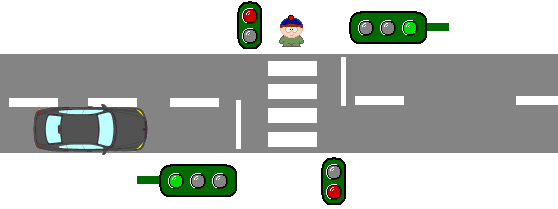
\includegraphics[width=0.8\linewidth]{../se-images/trafficlight.png}
  \caption{We will model a simple traffic light system.}
  \label{fig:trafficlight}
\end{figure}

% ==================================================================
\section{Tool Installation}
\label{sec:tutorial-tool-installation}
% ==================================================================

As of this writing, a complete toolchain is not yet available.  The following describes the installation from various components.

% ------------------------------------------------------------------
\subsection{Eclipse}
% ------------------------------------------------------------------

The basis for the toolchain are the \href{https://www.eclipse.org/downloads/packages/eclipse-modeling-tools/lunasr1}{Eclipse Modeling Tools}.  Please download for your platform and extract to a convenient location and start it.

\begin{info}
It may be not a bad idea to start with Polarsys instead, as it already includes Papyrus.
\end{info}

\begin{warning}On Linux, please edit eclipse.ini and add the following parameter \textbf{at the top (two lines}):

\begin{lstlisting}
--launcher.GTK_version
2
\end{lstlisting}
\end{warning}

% ------------------------------------------------------------------
\subsection{RMF and Formal Mind Essentials}
% ------------------------------------------------------------------

Next install the RMF (requirements) tools, but the repackaged version from Formal Mind:

\begin{itemize}
\item Use this update site: http://update.formalmind.com/studio
\item Unselect ``Group items by category''
\item Select \textbf{only} ``Formal Mind Studio (Feature)''
\item Complete the installation.
\end{itemize}

\begin{info}
The software is currently not signed, which will generate a warning.  Please continue with the installation, in spite of this.
\end{info}

% ------------------------------------------------------------------
\subsection{Java FX}
% ------------------------------------------------------------------

If you want to use rich text in requirements, you need support for Java FX.  Follow these steps:

\begin{itemize}
\item Use this update site: http://download.eclipse.org/efxclipse/runtime-released/1.1.0/site
\item Optional: Unselect ``Group items by category''
\item Select \textbf{only} ``Runtime Bundle Collector Feature''
\item Complete the installation.
\end{itemize}

% ------------------------------------------------------------------
\subsection{RMF-EMF Traceability}
% ------------------------------------------------------------------

In the context of a public research project (itea openETCS), a traceability plug-in for connecting arbitrary EMF models has been developed.

\begin{itemize}
\item Use this update site: http://openetcs.ci.cloudbees.com/job/openETCS-tycho/lastSuccessfulBuild/artifact/tool/bundles/org.openetcs.releng.products/target/repository
\item Unselect ``Group items by category''
\item Select \textbf{only} ``ProR Tracing Feature''
\item Complete the installation.
\end{itemize}

% ------------------------------------------------------------------
\subsection{Additional Modeling Components}
% ------------------------------------------------------------------

You can install additional components for modeling via \menu{Papyrus via Help | Install Modeling Components}.  For this tutorial, useful components include:

\begin{description}
\item[Ecore Tools.] Support diagram notation for Ecore models.
\item[Papyrus.] Supports UML and SysML.
\end{description}

We had some problems with installing the Ecore Tools.  If you cannot see a diagram in Section~\ref{}, then follow these steps:

Install software from this update site: http://download.eclipse.org/ecoretools/updates/releases/2.0.1/luna
Select Ecore Diagram Editor

% ------------------------------------------------------------------
\subsection{Team Support}
% ------------------------------------------------------------------

Eclipse supports a number of team environments.  We recommend the installation of the egit plugin, allowing to work with git repositories.  The installation is described in the \href{http://formalmind.com/handbook?page=sec-versioning.html}{formalmind Studio Handbook}.

% ------------------------------------------------------------------
\subsection{Tool Configuration}
% ------------------------------------------------------------------

We recommend to switch to the ProR perspective, to get started.

% ==================================================================
\section{Import Requirements}
% ==================================================================

Typically, you already have requirements available in some form.  ProR includes a simple CSV-Importer that allows you to import existing requirements.  Follow these steps:

\begin{itemize}
\item Create a new Project via \menu{File | New | Project... | General | Project}
\item Call it \menu{tdse-1}
\item Create a new Requirements Model via right-click on the project, selecting \menu{New | Reqif10 Model}
\item Call the Model \menu{Trafficlight.reqif}
\item Import the .csv file via \menu{File | Import | formalmind Studio | CSV}
\item Create a mapping for the two columns to String attributes, as shown in Figure~\ref{fig:csv-import}
\end{itemize}

\begin{figure}[h!]
  \centering
  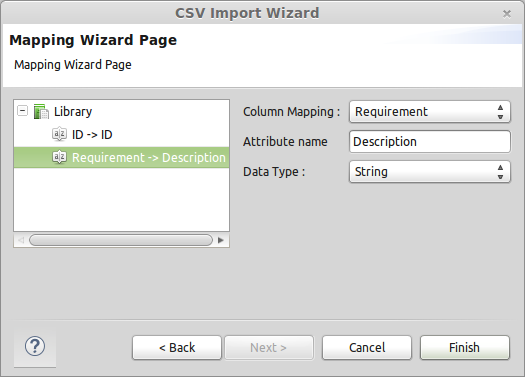
\includegraphics[width=\linewidth]{../se-images/csv-import.png}
  \caption{Result: The requirement is now a sibling of the chosen requirement.}
  \label{fig:csv-import}
\end{figure}

After the import, the new requirements have been added to the existing requirements specification.  There are a number of recommended improvements, for instance:

\begin{itemize}
\item Add a SpecObjectType for Headlines and configure the Headline Presentation, so that you can structure the text
\item Once you create headlines, you can arrange requirements as child elements (instead of siblings) under them.
\item You can create an information SpecObjectType, using XHTML and no IDs.  Use one of these to insert Figure~\ref{fig:trafficlight} into your specification (\href{../se-materials/tutorial/trafficlight.png}{trafficlight.png}).
\item Configure the ID Presentation to automatically create IDs for requirements, and center-align the ID.
\item Use the ID as a label (if available) by adjusting the Label Configuration.
\end{itemize}

The resulting specification is shown in Figure~\ref{fig:tutorial-step01}.

\begin{figure}[h!]
  \centering
  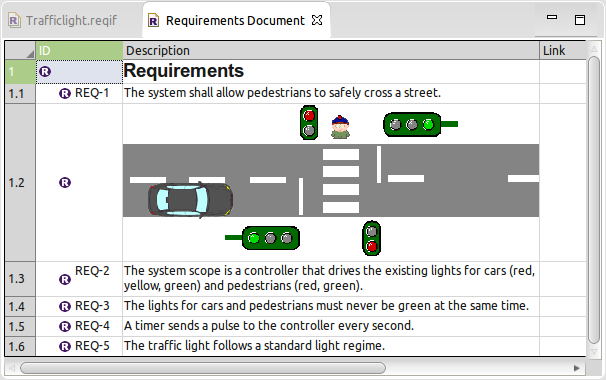
\includegraphics[width=\linewidth]{../se-images/tutorial-step01.png}
  \caption{The spec after completion of all steps so far.}
  \label{fig:tutorial-step01}
\end{figure}

% ==================================================================
\section{Glossary}
\label{sec:tutorial-glossary}
% ==================================================================

A glossary helps keeping track of terminology.  In this section, the glossary management from formalmind Studio is introduced, which supports color highlighting in the requirements text.

Note that this kind of glossary is a ``dead end'', in the sense that it cannot be used beyond its purpose.  Contrast that with a model-based data dictionary, as described in Section~\ref{sec:tutorial-ecore}.

The glossary is kind of cumbersome to configure.   Therefore, we included a correctly configured \href{../se-materials/tutorial/tdse-2/}{Sample Project}.  Note that you need both the Highlighting and Keyword Highlighting presentations, in that order.

Figure~\ref{fig:tutorial-step02} shows the glossary, and its application to the requirements, which have been rewritten to use the terminology of the specification.

\begin{figure}[h!]
  \centering
  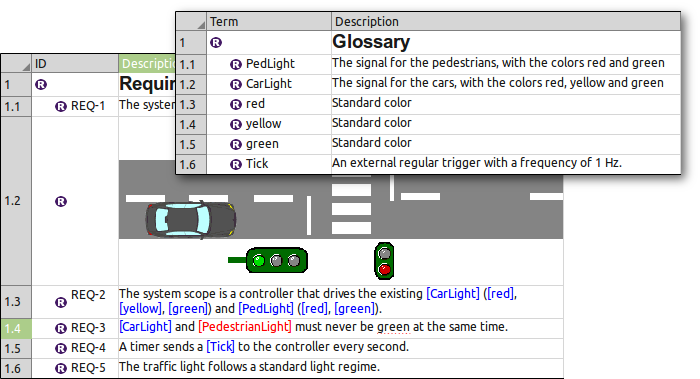
\includegraphics[width=\linewidth]{../se-images/tutorial-step02.png}
  \caption{Glossary Management in action.}
  \label{fig:tutorial-step02}
\end{figure}

In the screenshot, REQ-3 is being edited.  This results in the word \textit{green} being underlined in red, indicating that it is a recognized glossary entry.  The syntax highlighting diapears when not in edit mode.  Square brackets make a glossary term explicit.  If a term is marked that way that is not in the glossary, then it is shown in red.

% ==================================================================
\section{Data Dictionary with Ecore}
\label{sec:tutorial-ecore}
% ==================================================================

Ecore is the modeling language of the Eclipse Modeling Framework.  It has some similarities to UML Class diagrams, and is therefore well-suited for creating a precise data model.  It has the following advantages:

\begin{description}
\item[Easy to learn.] Especially if you already know class diagrams, you should be able to quickly learn Ecore.
\item[Code generation.] EMF allow the generation of Java code from Ecore models.  You can even generate a GUI based on a tree view.
\item[Test stub generation.] EMF allows the generation of test code stubs, making it easy to cover the unit test level.
\end{description}

On the other hand, it has its limitations.  In particular, it is not really possible to model dynamic aspects of the system.

\begin{warning}
While it is possible to mix this approach with the glossary management described in Section~\ref{sec:tutorial-glossary}, we do not recommend it, as it would lead to redundancy.  Redundancies should be avoided (DRY-principle: Don't Repeat Yourself).
\end{warning}

% ------------------------------------------------------------------
\subsection{Creating the Ecore Model}
% ------------------------------------------------------------------

We recommend to create a new Ecore Modeling Project via \menu{File | New | Project... | Eclipse Modeling Framework | Ecore Modeling Project}.   This way, everything will be properly configured for code generation and other cool stuff.  The model we use is shown in the right pane of Figure~\ref{fig:tutorial-step03}.

\begin{figure}[h!]
  \centering
  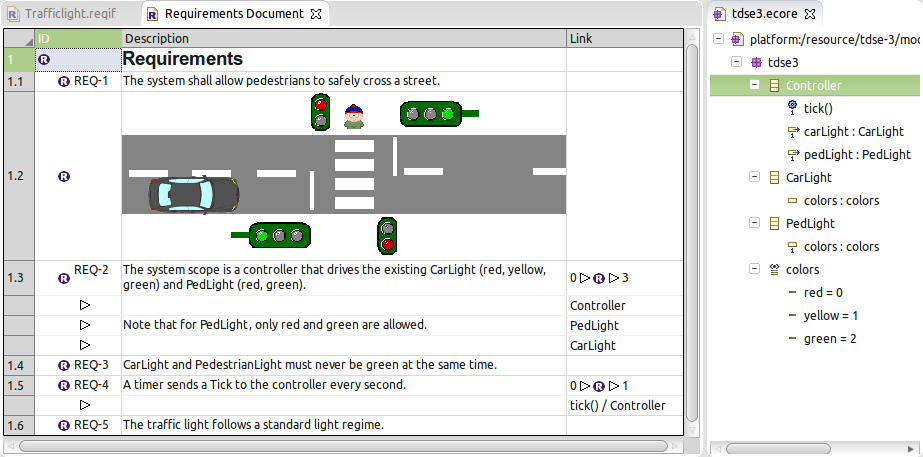
\includegraphics[width=\linewidth]{../se-images/tutorial-step03.png}
  \caption{On the left the requirements with links into the Ecore-based data model, shown on the right.}
  \label{fig:tutorial-step03}
\end{figure}

As you can see, the editors are arranged so that the requirements editor and the Ecore editor are visible at the same time.  This is necessary, as links are created by dragging model elements from the Ecore model onto the requirements.

\begin{info}
Linking via Drag and Drop is a feature taken from the openETCS project, \href{https://github.com/openETCS/toolchain/wiki/User-Documentation#Tracing_Requirements_and_SysML_Models}{where it is documented}.
\end{info}

We provided a preconfigured \href{../se-materials/tutorial/tdse-3/}{Sample Project}, that allows annotating traces, as also shown in Figure~\ref{fig:tutorial-step03} (the second link of REQ-2).

% ------------------------------------------------------------------
\subsection{Working with Diagrams}
% ------------------------------------------------------------------

Some people prefer diagrams to the tree-view shown in Figure~\ref{fig:tutorial-step03}, and diagrams can make communication easier.  If you installed the tool as described in Section~\ref{sec:tutorial-tool-installation}, then you can create a diagram from the Ecore model as described here.  Diagram and model will be synchronized, but it's possible to only show a subset of the model elements in the diagram.

A diagram should already have been created upon project creation.  You can open it by going to the Model Explorer or Project Explorer, and opening the .ecore model by clicking on the \[+\] to the left of the file name. it should show the package name (tdse3), and upon opening it again, it should unveal ``tdse3 class diagram''.  Doubleclicking should open the diagram editor, which will be empty, except instructions on how to add elements.

\begin{figure}[h!]
  \centering
  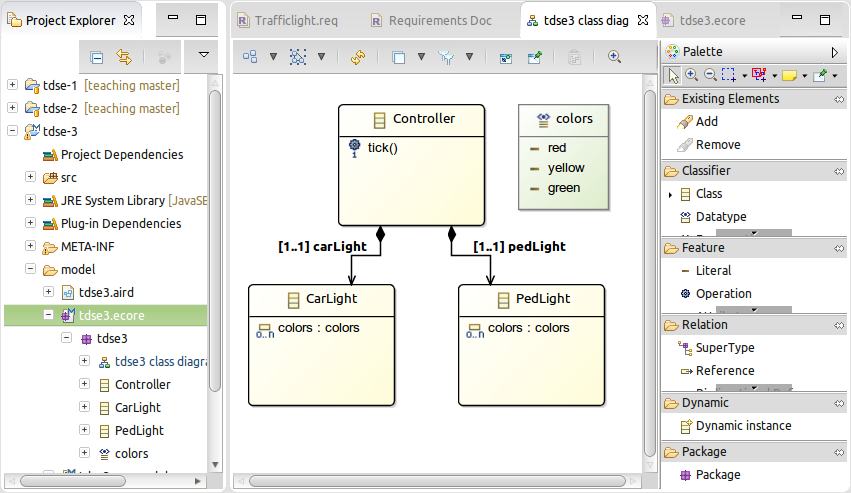
\includegraphics[width=\linewidth]{../se-images/ecore_diagram.png}
  \caption{The diagram has been created by dragging elements from the Project Explorer (left) to the drawing area (middle).  New elements can also be created by using the pallet on the right.}
  \label{fig:ecore_diagram}
\end{figure}

By dragging elements from the project explorer into the diagram area, we end up with the editor, as shown in Figure~\ref{fig:ecore_diagram}.  Elements and labels can be customized as one sees fit.  Changes to the model, including the creation of new elements, will be reflected in the tree view of the Ecore model as well.  Changes to the Ecore model will be seen here, but newly created elements will not appear on the diagram by default.  They have to be added manually.

\begin{itemize}
\item Right-click on the .ecore file and select \menu{Initialize Ecore Diagram...}
\item The correct .aird file should already be selected as the 
\end{itemize}

% ==================================================================
\section{Modeling with Papyrus}
% ==================================================================


